\section*{Podmínky, pomůcky a měřící přístroje}
Měření proběhlo při pokojové teplotě (přibližně \SI{25}{\degreeCelsius}) a normálním atmosférickém tlaku.

Jako oscilátor jsme použili permanentní magnet zavěšený na pružině.


Pod magnetem byla umístěna cívka připojená k počítači, který nám umožňoval do ní pouštět střídavé napětí o zvolené frekvenci a také zobrazovat časový průběh napětí indukované magnetem.


Indukované napětí by mělo být přibližně přímo úměrné okamžité rychlosti magnetu.
Periodu kmitu můžeme odečíst podle časové vzdálenosti jednotlivých peaků napětí.


Měřili jsme maximální napětí při pohybu magnetu nahoru i dolů.
Při pohybu dolů bylo napětí většinou výrazně vyšší (viz graf \ref{grp::mericipristroje}), takže předpokládáme, že měřící přístroj byl zatížen systematickou chybou.
Při měření konstanty tlumení se tuto chybu pokusíme odstranit tím, že u souboru naměřených peaků napětí nejdříve určíme střed jako průměr nulových a nenulových hodnot.
Dále vezmeme vzdálenost všech bodů od této hodnoty a až 
tento soubor hodnot prokládáme exponenciálou.

\begin{graph}[htbp] 
\centering
% GNUPLOT: LaTeX picture with Postscript
\begingroup
  \makeatletter
  \providecommand\color[2][]{%
    \GenericError{(gnuplot) \space\space\space\@spaces}{%
      Package color not loaded in conjunction with
      terminal option `colourtext'%
    }{See the gnuplot documentation for explanation.%
    }{Either use 'blacktext' in gnuplot or load the package
      color.sty in LaTeX.}%
    \renewcommand\color[2][]{}%
  }%
  \providecommand\includegraphics[2][]{%
    \GenericError{(gnuplot) \space\space\space\@spaces}{%
      Package graphicx or graphics not loaded%
    }{See the gnuplot documentation for explanation.%
    }{The gnuplot epslatex terminal needs graphicx.sty or graphics.sty.}%
    \renewcommand\includegraphics[2][]{}%
  }%
  \providecommand\rotatebox[2]{#2}%
  \@ifundefined{ifGPcolor}{%
    \newif\ifGPcolor
    \GPcolorfalse
  }{}%
  \@ifundefined{ifGPblacktext}{%
    \newif\ifGPblacktext
    \GPblacktexttrue
  }{}%
  % define a \g@addto@macro without @ in the name:
  \let\gplgaddtomacro\g@addto@macro
  % define empty templates for all commands taking text:
  \gdef\gplbacktext{}%
  \gdef\gplfronttext{}%
  \makeatother
  \ifGPblacktext
    % no textcolor at all
    \def\colorrgb#1{}%
    \def\colorgray#1{}%
  \else
    % gray or color?
    \ifGPcolor
      \def\colorrgb#1{\color[rgb]{#1}}%
      \def\colorgray#1{\color[gray]{#1}}%
      \expandafter\def\csname LTw\endcsname{\color{white}}%
      \expandafter\def\csname LTb\endcsname{\color{black}}%
      \expandafter\def\csname LTa\endcsname{\color{black}}%
      \expandafter\def\csname LT0\endcsname{\color[rgb]{1,0,0}}%
      \expandafter\def\csname LT1\endcsname{\color[rgb]{0,1,0}}%
      \expandafter\def\csname LT2\endcsname{\color[rgb]{0,0,1}}%
      \expandafter\def\csname LT3\endcsname{\color[rgb]{1,0,1}}%
      \expandafter\def\csname LT4\endcsname{\color[rgb]{0,1,1}}%
      \expandafter\def\csname LT5\endcsname{\color[rgb]{1,1,0}}%
      \expandafter\def\csname LT6\endcsname{\color[rgb]{0,0,0}}%
      \expandafter\def\csname LT7\endcsname{\color[rgb]{1,0.3,0}}%
      \expandafter\def\csname LT8\endcsname{\color[rgb]{0.5,0.5,0.5}}%
    \else
      % gray
      \def\colorrgb#1{\color{black}}%
      \def\colorgray#1{\color[gray]{#1}}%
      \expandafter\def\csname LTw\endcsname{\color{white}}%
      \expandafter\def\csname LTb\endcsname{\color{black}}%
      \expandafter\def\csname LTa\endcsname{\color{black}}%
      \expandafter\def\csname LT0\endcsname{\color{black}}%
      \expandafter\def\csname LT1\endcsname{\color{black}}%
      \expandafter\def\csname LT2\endcsname{\color{black}}%
      \expandafter\def\csname LT3\endcsname{\color{black}}%
      \expandafter\def\csname LT4\endcsname{\color{black}}%
      \expandafter\def\csname LT5\endcsname{\color{black}}%
      \expandafter\def\csname LT6\endcsname{\color{black}}%
      \expandafter\def\csname LT7\endcsname{\color{black}}%
      \expandafter\def\csname LT8\endcsname{\color{black}}%
    \fi
  \fi
  \setlength{\unitlength}{0.0500bp}%
  \begin{picture}(10204.00,6802.00)%
    \gplgaddtomacro\gplbacktext{%
      \csname LTb\endcsname%
      \put(682,3621){\makebox(0,0)[r]{\strut{} 0}}%
      \csname LTb\endcsname%
      \put(814,484){\makebox(0,0){\strut{} 0}}%
      \csname LTb\endcsname%
      \put(2313,484){\makebox(0,0){\strut{} 5}}%
      \csname LTb\endcsname%
      \put(3812,484){\makebox(0,0){\strut{} 10}}%
      \csname LTb\endcsname%
      \put(5311,484){\makebox(0,0){\strut{} 15}}%
      \csname LTb\endcsname%
      \put(6809,484){\makebox(0,0){\strut{} 20}}%
      \csname LTb\endcsname%
      \put(8308,484){\makebox(0,0){\strut{} 25}}%
      \csname LTb\endcsname%
      \put(9807,484){\makebox(0,0){\strut{} 30}}%
      \put(176,3620){\rotatebox{-270}{\makebox(0,0){\strut{}Výchylka}}}%
      \put(5310,154){\makebox(0,0){\strut{}Čas (\si{\s})}}%
    }%
    \gplgaddtomacro\gplfronttext{%
    }%
    \gplbacktext
    \put(0,0){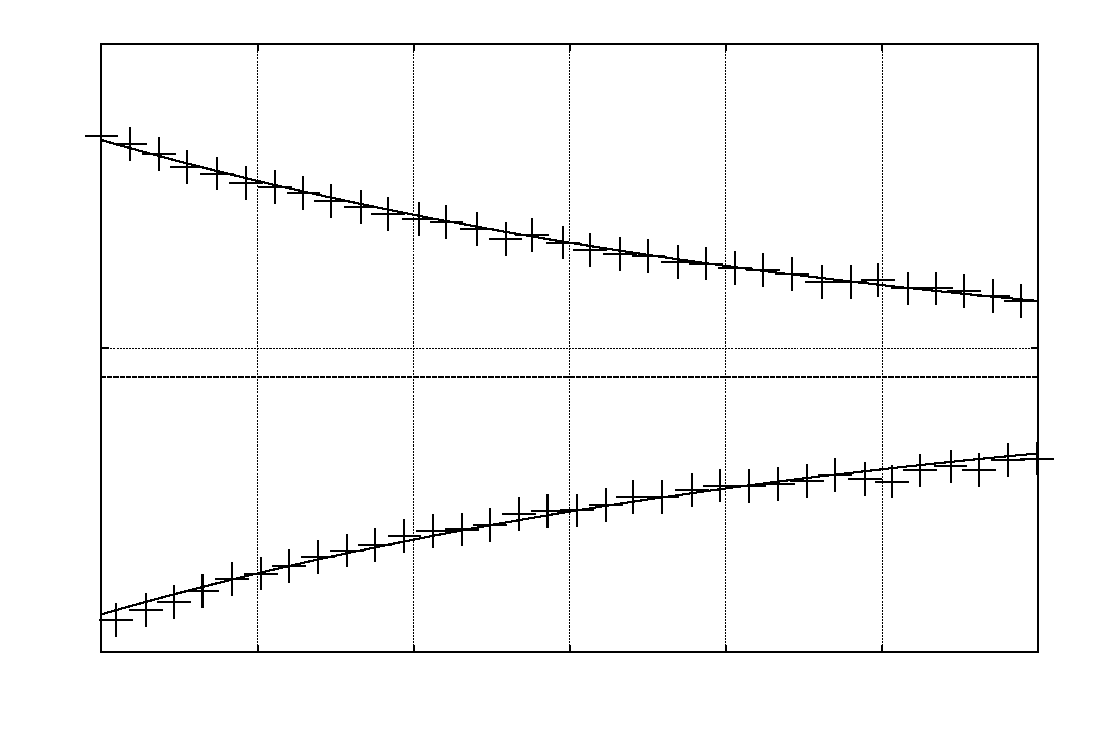
\includegraphics{tlumpuvodni}}%
    \gplfronttext
  \end{picture}%
\endgroup

\caption{Naměřené hodnoty při kmitání tlumeném modrým diskem, graf ilustruje způsob zpracování}
\label{grp::mericipristroje}
\end{graph}

Soustava nebyla kalibrovaná k měření výchylky, takže amplitudy u nuceného kmitání uvádíme pouze v poměru k nejvyšší naměřené hodnotě.
Při pohybu dolů bylo napětí opět vyšší, relativní velikost výchylky určíme jako rozdíl průměru kladných maxim a průměru záporných maxim (viz graf \ref{grp::nucenyilustrace}).

\begin{graph}[htbp] 
\centering
% GNUPLOT: LaTeX picture with Postscript
\begingroup
  \makeatletter
  \providecommand\color[2][]{%
    \GenericError{(gnuplot) \space\space\space\@spaces}{%
      Package color not loaded in conjunction with
      terminal option `colourtext'%
    }{See the gnuplot documentation for explanation.%
    }{Either use 'blacktext' in gnuplot or load the package
      color.sty in LaTeX.}%
    \renewcommand\color[2][]{}%
  }%
  \providecommand\includegraphics[2][]{%
    \GenericError{(gnuplot) \space\space\space\@spaces}{%
      Package graphicx or graphics not loaded%
    }{See the gnuplot documentation for explanation.%
    }{The gnuplot epslatex terminal needs graphicx.sty or graphics.sty.}%
    \renewcommand\includegraphics[2][]{}%
  }%
  \providecommand\rotatebox[2]{#2}%
  \@ifundefined{ifGPcolor}{%
    \newif\ifGPcolor
    \GPcolorfalse
  }{}%
  \@ifundefined{ifGPblacktext}{%
    \newif\ifGPblacktext
    \GPblacktexttrue
  }{}%
  % define a \g@addto@macro without @ in the name:
  \let\gplgaddtomacro\g@addto@macro
  % define empty templates for all commands taking text:
  \gdef\gplbacktext{}%
  \gdef\gplfronttext{}%
  \makeatother
  \ifGPblacktext
    % no textcolor at all
    \def\colorrgb#1{}%
    \def\colorgray#1{}%
  \else
    % gray or color?
    \ifGPcolor
      \def\colorrgb#1{\color[rgb]{#1}}%
      \def\colorgray#1{\color[gray]{#1}}%
      \expandafter\def\csname LTw\endcsname{\color{white}}%
      \expandafter\def\csname LTb\endcsname{\color{black}}%
      \expandafter\def\csname LTa\endcsname{\color{black}}%
      \expandafter\def\csname LT0\endcsname{\color[rgb]{1,0,0}}%
      \expandafter\def\csname LT1\endcsname{\color[rgb]{0,1,0}}%
      \expandafter\def\csname LT2\endcsname{\color[rgb]{0,0,1}}%
      \expandafter\def\csname LT3\endcsname{\color[rgb]{1,0,1}}%
      \expandafter\def\csname LT4\endcsname{\color[rgb]{0,1,1}}%
      \expandafter\def\csname LT5\endcsname{\color[rgb]{1,1,0}}%
      \expandafter\def\csname LT6\endcsname{\color[rgb]{0,0,0}}%
      \expandafter\def\csname LT7\endcsname{\color[rgb]{1,0.3,0}}%
      \expandafter\def\csname LT8\endcsname{\color[rgb]{0.5,0.5,0.5}}%
    \else
      % gray
      \def\colorrgb#1{\color{black}}%
      \def\colorgray#1{\color[gray]{#1}}%
      \expandafter\def\csname LTw\endcsname{\color{white}}%
      \expandafter\def\csname LTb\endcsname{\color{black}}%
      \expandafter\def\csname LTa\endcsname{\color{black}}%
      \expandafter\def\csname LT0\endcsname{\color{black}}%
      \expandafter\def\csname LT1\endcsname{\color{black}}%
      \expandafter\def\csname LT2\endcsname{\color{black}}%
      \expandafter\def\csname LT3\endcsname{\color{black}}%
      \expandafter\def\csname LT4\endcsname{\color{black}}%
      \expandafter\def\csname LT5\endcsname{\color{black}}%
      \expandafter\def\csname LT6\endcsname{\color{black}}%
      \expandafter\def\csname LT7\endcsname{\color{black}}%
      \expandafter\def\csname LT8\endcsname{\color{black}}%
    \fi
  \fi
  \setlength{\unitlength}{0.0500bp}%
  \begin{picture}(5668.00,4534.00)%
    \gplgaddtomacro\gplbacktext{%
      \csname LTb\endcsname%
      \put(418,2377){\makebox(0,0)[r]{\strut{}}}%
      \put(550,264){\makebox(0,0){\strut{}}}%
      \put(1337,264){\makebox(0,0){\strut{}}}%
      \put(2124,264){\makebox(0,0){\strut{}}}%
      \put(2911,264){\makebox(0,0){\strut{}}}%
      \put(3697,264){\makebox(0,0){\strut{}}}%
      \put(4484,264){\makebox(0,0){\strut{}}}%
      \put(5271,264){\makebox(0,0){\strut{}}}%
      \put(176,2376){\rotatebox{-270}{\makebox(0,0){\strut{}Napětí}}}%
      \put(2910,154){\makebox(0,0){\strut{}Čas (\si{\s})}}%
    }%
    \gplgaddtomacro\gplfronttext{%
    }%
    \gplbacktext
    \put(0,0){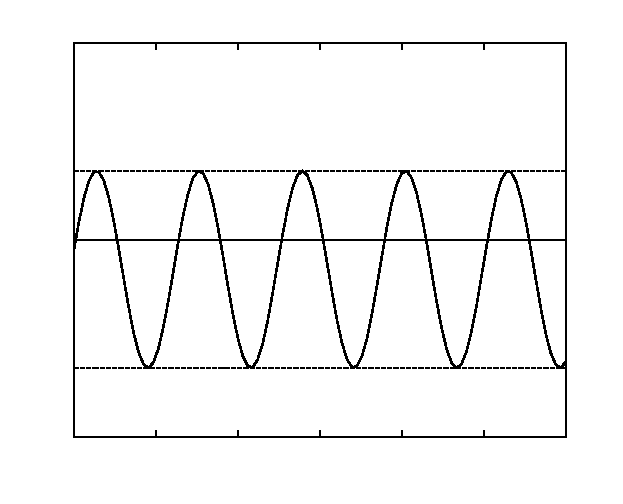
\includegraphics{nucenyilustrace}}%
    \gplfronttext
  \end{picture}%
\endgroup

\caption{Ilustrace metody určení amplitudy při nucených kmitech, poměrnou amplitudu určíme jako vzdálenost dvou čárkovaných přímek}
\label{grp::nucenyilustrace}
\end{graph}